\chapter{\selectlanguage{greek}Εισαγωγή}
Ο σκοπός κάθε συστήματος επικοινωνίας είναι η μετάδοση πληροφορίας απο την πηγή σε κάποιον προορισμό μέσω ενός καναλιού επικοινωνίας. Το πρωτεύον πρόβλημα αυτής της διαδικασίας, ορίστηκε από τον \en{Claude E. Shannon} στην καθοριστική εργασία του το 1948, ως η αναπαραγωγή σε ένα σημείο ενός μηνύματος που επιλέγεται σε άλλο σημείο, κατά το δυνατόν ακριβής. Ο σχεδιασμός του τηλεπικοινωνιακού συστήματος πρέπει να είναι τέτοιος, ώστε αυτό να λειτουργεί για κάθε δυνατή επιλογή μηνύματος πληροφορίας, μιας και τη στιγμή σχεδιασμού το ακριβές αυτό μήνυμα δεν είναι γνωστό \cite{shannon1948mathematical}.

\begin{figure}[h]
\center{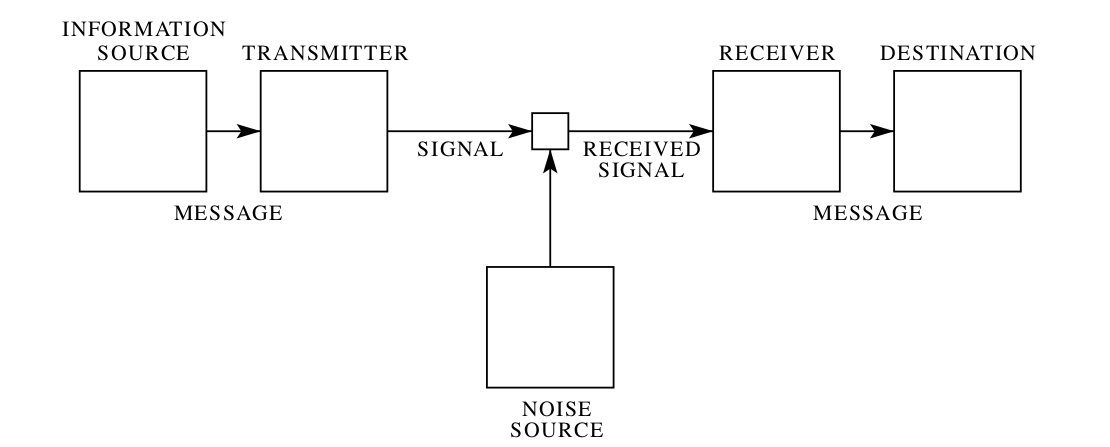
\includegraphics[width=0.75\linewidth]{figures/comm_system.png}}
\caption{Σχηματικό διάγραμμα τυπικού τηλεπικοινωνιακού συστήματος}
\label{fig:telecom system}
\end{figure}

Στο παραπάνω σχήμα (Σχήμα \ref{fig:telecom system}), φαίνεται το μπλοκ διάγραμμα ενός τυπικού τηλεπικοινωνιακού συστήματος, και τα βασικά μέρη από τα οποία αποτελείται: την πηγή πληροφορίας, τον πομπό, όπου γίνεται μετατροπή του μηνύματος πληροφορίας σε σήμα κατάλληλο για μετάδοση, το κανάλι, μέσω του οποίου γίνεται η μετάδοση, τον δέκτη, όπου γίνεται λήψη του σήματος και ανάκτηση του αρχικού μηνύματος και τέλος, τον τελικό προορισμό της πληροφορίας.

Tα κύρια μέρη από τα οποία αποτελείται το τηλεπικοινωνιακό σύστημα που περιγράφηκε, φαίνονται αναλυκτικότερα στο Σχήμα \ref{fig:telecom system 2}. Tο στάδιο της κωδικοποίησης πηγής (\en{source encoding}) δεν μας απασχολεί, οπότε και θεωρείται πως η πηγή εκπέμπει μια διακριτή ακολουθία από ανεξάρτητα και ομοιόμορφα κατανεμημένα (\en{independent \& identically distributed - i.i.d.}) σύμβολα, τα οποία εισάγονται στον κωδικοποιητή καναλιού.

\begin{figure}[h]
\center{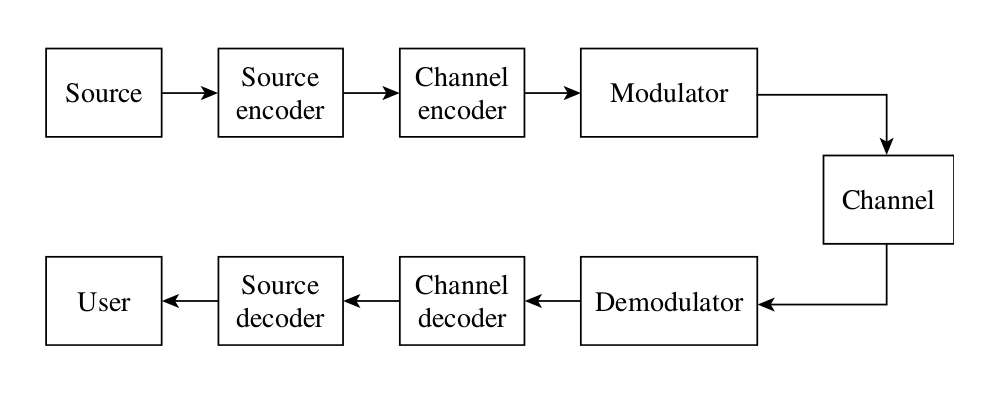
\includegraphics[width=0.8\linewidth]{figures/comm_system_2.png}}
\caption{Κύρια μέρη του τηλεπικοινωνιακού συστήματος}
\label{fig:telecom system 2}
\end{figure}

\subsection*{Το κανάλι επικοινωνίας}
Ένα κανάλι επικοινωνίας μπορεί είναι οποιοδήποτε μέσο μέσα στο οποίο η πληροφορία μπορεί να αποθηκευτεί ή μέσω του οποίου μπορεί να μεταδοθεί. Στα πλαίσια του τηλεπικοινωνιακού συστήματος, το τηλεπικοινωνιακό κανάλι ορίζεται ως ο χώρος που μεσολαβεί ανάμεσα στον πομπό και τον δέκτη και στον οποίο λαμβάνει χώρα η μετάδοση πληροφορίας. Σε θεωρητικό επίπεδο, το κανάλι αποτελεί τη μαθηματική αφαίρεση των ειδών και της έντασης του θορύβου που αλλοιώνει τη μεταδιδόμενη πληροφορία.

\begin{figure}[h]
\center{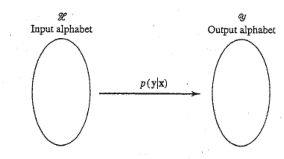
\includegraphics[width=0.7\linewidth]{figures/discrete_channel.png}}
\caption{Το διακριτό κανάλι}
\label{fig:discrete channel}
\end{figure}

Η είσοδος και η έξοδος των καναλιών που συναντάμε στην πράξη είναι εν γένει σήματα διακριτού-χρόνου. Στην περίπτωση που οι μεταβλητές εισόδου-εξόδου είναι πεπερασμένες ή άπειρα αριθμήσιμες, το κανάλι καλείται \textit{διακριτό} (\en{discrete channel}). Το διακριτό κανάλι, το σχηματικό διάγραμμα του οποίου φαίνεται στο Σχήμα \ref{fig:discrete channel}, ορίζεται ως εξής:

\begin{definition}
Ένα διακριτό κανάλι, συμβολίζεται ως ($\mathcal{X},\;p(x\mid{y}),\;\mathcal{Y}$), και αποτελείται από δύο πεπερασμένα σύνολα (\en{finite sets}) $\mathcal{X}$ και $\mathcal{Y}$, καθώς και μια συλλογή συναρτήσεων πυκνότητας πιθανότητας $p(x\mid{y})$, μία για κάθε $x\in\mathcal{X}$, τέτοιες ώστε, για κάθε $x$, $y$ να ισχύει $p(y\mid{x})\ge0$ και $\sum\nolimits_{y}p(y\mid{x})=1\;\;\forall{x}$, όταν $\mathcal{X}$ είναι η είσοδος και $\mathcal{Y}$ η έξοδος του καναλιού. \\
\cite{cover2012elements}, \cite{proakis1994communication}
\label{def:discrete channel}
\end{definition}

\begin{figure}[h]
\center{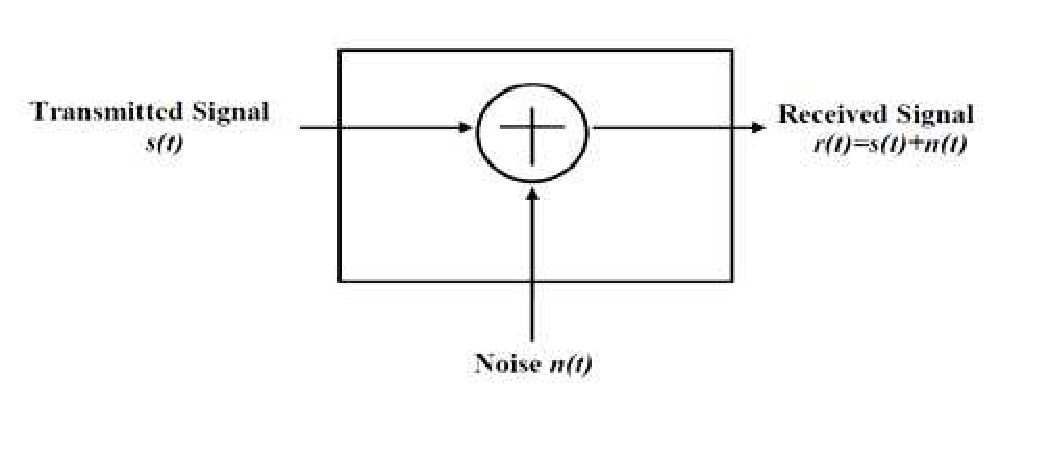
\includegraphics[width=0.8\linewidth]{figures/awgn_channel.eps}}
\caption{Κανάλι \en{AWGN} θορύβου}
\label{fig:awgn channel}
\end{figure}

Όπως φαίνεται στο Σχήμα \ref{fig:awgn channel}, στο μεταδιδόμενο σήμα $s(t)$ προστίθεται ο θόρυβος που εισάγεται κατά τη μετάδοση από το κανάλι και αποτελεί αναπόδραστη αιτία υποβάθμισης του σήματος πληροφορίας. Ο θόρυβος εκτός από προσθετικός, μοντελοποιείται ως λευκός (ίση πυκνότητα ισχύος σε όλο το φάσμα συχνοτήτων), \en{Gaussian} (ακολουθεί την κανονική ή γκαουσσιανή κατανομή στο πεδίο του χρόνου) θόρυβος (\en{Additive White Gaussian Noise, AWGN)}.

\section{Το θεώρημα \en{Shannon}}
Ο κύριος στόχος του τηλεπικοινωνιακού συστήματος είναι η αξιόπιστη μετάδοση πληροφορίας, μέσω του καναλιού επικοινωνίας και η σωστή ανάκτησή της στο δέκτη. Ένα βασικό αποτέλεσμα της θεωρίας πληροφοριών είναι ότι, ακόμη και με την παρουσία θορύβου, είναι δυνατό να επιτευχθεί αξιόπιστη μετάδοση αρκέι ο ρυθμός αποστολής πληροφορίας να είναι μικρότερος από ένα δεδομένο κατώφλι. Το παρακάτω θεώρημα, αποδείχθηκε από τον \en{Shannon} και αποτελεί θεμελιώδες θεώρημα της θεωρίας τηλεπικοινωνιών:

\begin{theorem}(Θεώρημα Κωδικοποίησης Ενθόρυβου Καναλιού)
Ο ρυθμός αποστολής πληροφορίας μέσω του τηλεπικοινωνιακού συστήματος έχει μέγιστο \en{C}, που καλείται \textbf{χωρητικότητα καναλιού}
\begin{itemize}
\item Όταν ισχύει:
\begin{equation}
R\leq{C}
\end{equation}
,όπου $R$ ο ρυθμός αποστολής της πληροφορίας (\en{bits} ανά χρήση του καναλιού), τότε υπάρχει τεχνική κωδικοποίησης καναλιού, έτσι ώστε να είναι δυνατή μετάδοση με αυθαίρετα μικρό σφάλμα.
\item Στην αντίθετη περίπτωση η αξιοπιστία της επικοινωνίας δεν μπορεί να ελεγχθεί.
\end{itemize}
\label{theorem:shannon}
\end{theorem}


Αξίζει να σημειωθεί πως, ενώ το θεώρημα \en{Shannon} αποδεικνύει, για οποιοδήποτε ρυθμό μικρότερο της χωρητικότητας την ύπαρξη τεχνικών κωδικοποίησης, κατάλληλων ώστε να υπάρχει οσοδήποτε μικρό σφάλμα κατά την επικοινωνία, η απόδειξη δεν είναι κατασκευαστική (\en{constructive}), δηλαδή δεν προτείνεται κάποιος συγκεκριμένος κώδικας. Ακόμη, από το θεώρημα προκύπτει πως ο βασικός περιορισμός που θέτει ο θόρυβος σε ένα κανάλι επικοινωνίας αφορά το ρυθμό μετάδοσης δεδομένων και όχι την αξιοπιστία της επικοινωνίας \cite{proakis1994communication}, \cite{shannon1948mathematical}.

\section{Τυχαίοι κώδικες - Πολυπλοκότητα}
\begin{definition}{Κώδικας $C(n,M)$}

Ένας κώδικας $C(n,M)$ για ένα διακριτό κανάλι που προκύπτει από τον Ορισμό \ref{def:discrete channel}, αποτελείται από τα εξής στοιχεία:
\begin{itemize}
\item Ένα σύνολο δεικτών $[1, 2, \ldots, M]$ 
\item Μια συνάρτηση κωδικοποίησης $X^n:\left\lbrace1, 2, \ldots, M\right\rbrace\to\mathcal{X}^n$ η οποία παράγει τις κωδικές λέξεις $x^n\left(1\right), x^n\left(2\right), \ldots, x^n\left(M\right)$. Το σύνολο των κωδικών λέξεων, καλείται \textit{κωδικό βιβλίο}
\item Μια συνάρτηση αποκωδικοποίησης $g:\mathcal{Y}^n\to\left\lbrace1, 2, \ldots, M\right\rbrace$ η οποία λειτουργεί ως ένας ντετερμινιστικός κανόνας, που αποδίδει μια πρόβλεψη σε κάθε ληφθέν διάνυσμα
\end{itemize}
\label{def:code}
\end{definition}

Στο εξής, όταν αναφέρεται κώδικας, θα εννοείται το κωδικό βιβλίο του, το οποίο θα συμβολίζεται ως $C(n,M)$. Θα χρειαστεί να σημειωθεί, όπως αναφέρθηκε και στην προηγούμενη παράγραφο πως, ενώ το θεώρημα \en{Shannon} αποδεικνύει την ύπαρξη κωδίκων που πλησιάζουν τη χωρητικότητα, δεν προτείνει κάποια συγκεκριμένη επιλογή βέλτιστου κώδικα.

Η ρητή κατασκευή (\en{explicit construction}) \enquote*{καλών} κωδίκων αποτελεί δύσκολο έργο. Αντί αυτής, η τυπική προσέγγιση βασίζεται στην πιθανοτική μέθοδο (\en{probabilistic method}) και προβλέπει πως σε ένα σύνολο κωδίκων οι οποίοι έχουν κατασκευαστεί με τυχαίο τρόπο, η πιθανότητα να υπάρχουν καλοί κώδικες εντός του είναι θετική. Για την ακρίβεια, κάνοντας χρήση κάποιας ανισότητας συγκέντρωσης (π.χ. ανισότητα \en{Markov}), αποδεικνύεται πως η πιθανότητα να επιλεγεί ένας καλός κώδικας μέσα από αυτό το σύνολο τείνει στο 1, καθώς το μήκος του κώδικα $n$ μεγαλώνει. Στη συνέχεια θα οριστεί ένας τυχαίος κώδικας που ικανοποιεί το Θεώρημα \ref{theorem:shannon} και θα εξεταστεί ο τρόπος κατασκευής του και η πολυπλοκότητα την οποία εισάγει η χρήση του.

\subsection{Τυχαίοι κώδικες}
Ένα σώμα πεπερασμένου αριθμού στοιχείων (\en{finite field}) $\mathbb{F}_q$, είναι ένα σύνολο από στοιχεία των οποίων το άθροισμα και το γινόμενο, είναι επίσης στοιχεία του συνόλου. Επίσης, η πρόσθεση κι ο πολλαπλασιασμός στοιχείων ικανοποιούν την αντιμεταθετική, προσεταιριστική, και επιμεριστική ιδιότητα. Tο πλήθος των στοιχείων ενός σώματος συμβολίζεται ως $|\mathbb{F}_q|$. Ευρέως χρησιμοποιούμενο είναι το \textit{δυαδικό} σώμα $\mathbb{F}_2$ το οποίο αποτελείται από τα στοιχεία \{0,1\}, επομένως ισχύει $|\mathbb{F}_2|=2$. Το σώμα αυτό θα υποθέτουμε και σε όλη την έκταση της παρούσας εργασίας.


Χρησιμοποιώντας τη σημειολογία του Ορισμού \ref{def:code}, καθώς και το σώμα $\mathbb{F}_2$, ο \textit{ρυθμός κώδικα} $C(n,M)$ (ρυθμός αποστολής πληροφορίας) ορίζεται από την παρακάτω εξίσωση:
\begin{equation}
R=\frac{\log_{2}M}{n}\;\;\;\;(bits/transmission)
\label{eq: code rate}
\end{equation}
\cite{cover2012elements}.

Η κατασκευή τυχαίων κωδίκων επί του σώματος $\mathbb{F}_2$, ακολουθεί την εξής διαδικασία:
\begin{definition}{(Τυχαίο σύνολο \en{Shannon}).}

Το σύνολο όλων των κωδίκων $C(n,M)$ μήκους $n$ και πληθυκότητας $M$ αποτελείται από $|\mathbb{F}|_2^{nM}$ δυνατούς κώδικες, καθώς υπάρχουν $nM$ βαθμοί ελευθερίας στην επιλογή κάθε στοιχείου του κωδικού βιβλίου. Στα στοιχεία του συνόλου προσδίδεται η ομοιόμορφη κατανομή πιθανότητας και επιλέγονται τυχαία τα στοιχεία $x^{[1]},...,x^{[M]}$ του συνόλου. \cite{richardson2008modern},\cite{shannon1948mathematical}
\label{def:random_ensemble}
\end{definition}

\subsection{Πολυπλοκότητα}
Είναι προφανές πως, οι (τυχαίοι) κώδικες που προκύπτουν από τον Ορισμό \ref{def:random_ensemble} ικανοποιούν και το θεώρημα \en{Shannon}, είναι δηλαδή ικανοί να λειτουργήσουν κοντά στη χωρητικότητα, με αυθαίρετα μικρό σφάλμα. Παρά το ότι η τυχαία κωδικοποίηση αποτελεί την προφανή λύση στο πρόβλημα κωδικοποίσης, υστερεί σε δυνατότητα πρακτικής υλοποίησης, καθώς δεν λαμβάνει υπ'όψιν την πολυπλοκότητα αποθήκευσης του κώδικα (πολυπλοκότητα περιγραφής) και την πολυπλοκότητα κωδικοποίησης και αποκωδικοποίησης.

Στην περίπτωση ενός κώδικα που προκύπτει από τον Ορισμό \ref{def:random_ensemble}, προκύπτει εύκολα πως η πολυπλοκότητα αποθήκευσης είναι εκθετική με το μήκος του κώδικα, καθώς απαιτούνται $nM = n\*2^{Rn}$ \en{bits} για την αποθήκευση του κωδικού βιβλίου $C(n,M)$ στον κωδικοποιητή, για τη σύνθεση του μηνύματος που θα εισέλθει για μετάδοση από το κανάλι. Ακόμη ο αποκωδικοποιητής θα πρέπει να έχει αποθηκευμένη κάθε δυνατή κωδική λέξη και (όπως ήδη αναφέρθηκε) να εκτελέσει αναζήτηση για τον έλεγχο και την απόφαση του μηνύματος πληροφορίας που στάλθηκε. Παρατηρείται συνεπώς, πως με την αύξηση του μήκους \en{n} η πολυπλοκότητα καθίσταται απαγορευτική.

Συνοψίζοντας, διαπιστώνεται πως το πρόβλημα έγκειται στη δυνατότητα προσέγγισης της χωρητικότητας με πρακτικό τρόπο.

\subsection{Πρακτικοί κωδικοποιητές/αποκωδικοποιητές}
Τη δυνατότητα αυτοί δίνουν διαδικασίες κωδικοποίησης (\en{coding schemes}) και αποκωδικοποίσης, σχεδιασμένες με γνώμονα τη δυνατότητα πρακτικής υλοποίησης. Οι κώδικες που προκύπτουν διακρίνονται από δομικές αλγεβρικές ιδιότητες και ορίζονται από συγκεκριμένους κανόνες για την κωδικοποίηση και την αποκωδικοποίηση.

Θα αποδειχθεί στη συνέχεια της εργασίας, πως με έναν τέτοιο τρόπο, η πολυπλοκότητα κωδικοποίησης και αποκωδικοποίησης απλοποιείται σημαντικά, και καταλήγει να είναι τετραγωνικής ($\mathcal{O}(n^2)$) ή και γραμμικής ($\mathcal{O}(n)$) τάξης.Οι αλγεβρικές δομικές ιδιότητες προσδίδονται στους κώδικες για ακριβώς το σκοπό αυτό. Θα οριστούν επίσης έννοιες όπως οι αραιοί πίνακες, η επαναληπτική αποκωδικοποίηση και τα γραφήματα \en{Tanner} ως εργαλεία για την περιγραφή τέτοιων κωδίκων.

\section{Δομή εργασίας}
Η εργασία θα ακολουθήσει την εξής δομή: Στο Κεφάλαιο 2 θα αναλυθούν οι αλγεβρικές δομικές ιδιότητες των κωδίκων καναλιού, ώστε να καταστεί πρακτική η κωδικοποίηση και αποκωδικοποίηση τους και θα οριστούν οι γραμμικοί μετασχηματισμοί για την εκτέλεσή τους, οι πίνακες \textbf{\en{G}} και \textbf{\en{H}}. Στο Κεφάλαιο 3 θα οριστούν και θα περιγραφούν οι κώδικες επανάληψης - συσσώρευσης (\en{repeat-accumulate}) ως υποομάδα τόσο των κωδίκων \en{turbo} όσο και των \en{LDPC} κωδίκων και θα εξεταστεί ο μηχανισμός και η πολυπλοκότητα κωδικοποίησης και αποκωδικοποίησής τους. Στο Κεφάλαιο 4 θα περιγραφεί αναλυτικά η προσομοίωση που έγινε και θα παρουσιαστούν τα αποτελέσματά της. Τέλος στο Κεφάλαιο 5 θα παρουσιαστούν οι δυνατότητες περαιτέρω μελέτης καθώς και πρόσθετες επεκτάσεις, στηριζόμενες στη γλωσσα \en{C}\texttt{++} και \en{CUDA C}.
